\documentclass[11pt,a4paper]{article}
\usepackage[margin=3cm]{geometry}
\usepackage[utf8]{inputenc}
\usepackage{courier}
\usepackage{amsmath}
\usepackage{amsfonts}
\usepackage{amssymb}
\usepackage{makeidx}
\usepackage{graphicx}
\usepackage{hyperref}
\usepackage{indentfirst}
\usepackage{xcolor}
\usepackage{epsfig}
\usepackage{listings}
% -- subtitle
\usepackage{titling}
\newcommand{\subtitle}[1]{%
	\posttitle{%
		\par\end{center}
	\begin{center}\large#1\end{center}
	\vskip0.5em}%
    % http://tex.stackexchange.com/questions/50182/subtitle-with-the-maketitle-page
}
% -- fonts
\usepackage{fontspec}
\setmainfont{RomanSerif}
\setsansfont{Overlock}
\setmonofont{Inconsolata}
% -- xmark
\newcommand{\xmark}{\textcolor{green!50!black}{x}}
% -- table font size -- http://tex.stackexchange.com/questions/27097/changing-the-font-size-in-a-table
\usepackage{floatrow}
\DeclareFloatFont{large}{\large} % "scriptsize" is defined by floatrow, "tiny" not
\floatsetup[table]{font=large}
% -- author, title
\author{}
\title{24+Radio Catalog Manual}
\subtitle{(GOODS-North)}
\begin{document}
\maketitle
\tableofcontents
\clearpage
\setlength{\baselineskip}{16pt}
\setlength{\parskip}{5pt}
% -- code style text box
\lstset{
	numbers=left,
	stepnumber=1,
	numbersep=10pt,
	numberstyle=\footnotesize,
	basicstyle=\fontsize{8}{12}\ttfamily,
	keywordstyle=\color{blue!70},
	commentstyle=\color{red!50!green!50!blue!50},
	frame=shadowbox,
	rulesepcolor=\color{red!20!green!20!blue!20},
	escapeinside=``,
	xleftmargin=2em,
	xrightmargin=0em,
	aboveskip=1em,
	tabsize=4,
	showspaces=false,
	showstringspaces=false
}

%*************************************************************************************
\section{Abstract}

This is the manual for the 24+radio catalog. We select sources from the GOODS-Spitzer IRAC catalog in GOODS-North field using 24 and radio images. 

We use Monte-Carlo simulation to validate and correct measurements. The output is a catalog contains IRAC, Ks, 24 and radio band flux and uncertainties. Additional, we measure 16um based on this catalog, and append 16um flux and uncertainty to our final 24+radio catalog. 

With the final 24+radio catalog, we do a panchromatic SED fitting to derive SFR, dust mass, and to predict the far-infrared band fluxes, which will be used for the next step ''super-deblending'' photometry. 

\vspace{5cm}
Hints: black text are our method and procedures, \textcolor{blue}{blue text are notes}, and \textcolor{red}{red text are unsolved issues.}

%*************************************************************************************

\clearpage

%*************************************************************************************
\section{Band 24}

\subsection{Galfit at band 24}

We use these commands to run the galfit photometry at band 24:

\begin{lstlisting}[language=bash]
# run first-pass without varying source position
./do_Galfit 24 201500 -catalog irac_mips_fluxes_hdfn.dat
cd boxgalfit; do_GalfitRunqsub; cd ..
./do_Galfit 24 201500 -catalog irac_mips_fluxes_hdfn.dat -postparallel
# then second-pass varying source position
./do_Galfit 24 201500 -catalog irac_mips_fluxes_hdfn.dat -vary
cd boxgalfit_vary; do_GalfitRunqsub; cd ..
./do_Galfit 24 201500 -catalog irac_mips_fluxes_hdfn.dat -vary -postparallel
\end{lstlisting}

\subsection{Galsim at band 24}

We use these commands to run the Monte-Carlo simulation at band 24:

\begin{lstlisting}[language=bash]
# first estimate magnitude range
convert_flux2mag goodsn 24 $(0.0044*01) 1 # (mBias -0.2036 fBias -0.000553)
convert_flux2mag goodsn 24 $(0.0044*25) 1 # (mBias -0.2036 fBias -0.000553)
# then do the simulation
# ./do_Galsim 24 201500 -mag0 -2.8416 -mag1 0.530157 -number 6000 -vary \
-catalog RadioOwenMIPS24_priors_April18_2014.txt
./do_Galsim 24 201500 -mag0 -2.8416 -mag1 0.530157 -number 6000 -vary \
-catalog irac_mips_fluxes_hdfn.dat
cd boxgalsim; do_GalsimRunqsub; cd ..
./do_Galsim 24 201500 -mag0 -2.8416 -mag1 0.530157 -number 6000 -vary \
-catalog irac_mips_fluxes_hdfn.dat -postparallel
\end{lstlisting}

\subsection{Galsim Analysis at band 24}

We use these commands to run the simulation analysis at band 24:

\begin{lstlisting}[language=bash]
sm
macro read run_simu_stats_v7.sm run_simu_stats_v7 24 201500
\end{lstlisting}

Below are our statistical analyses:

\begin{figure}[H]
	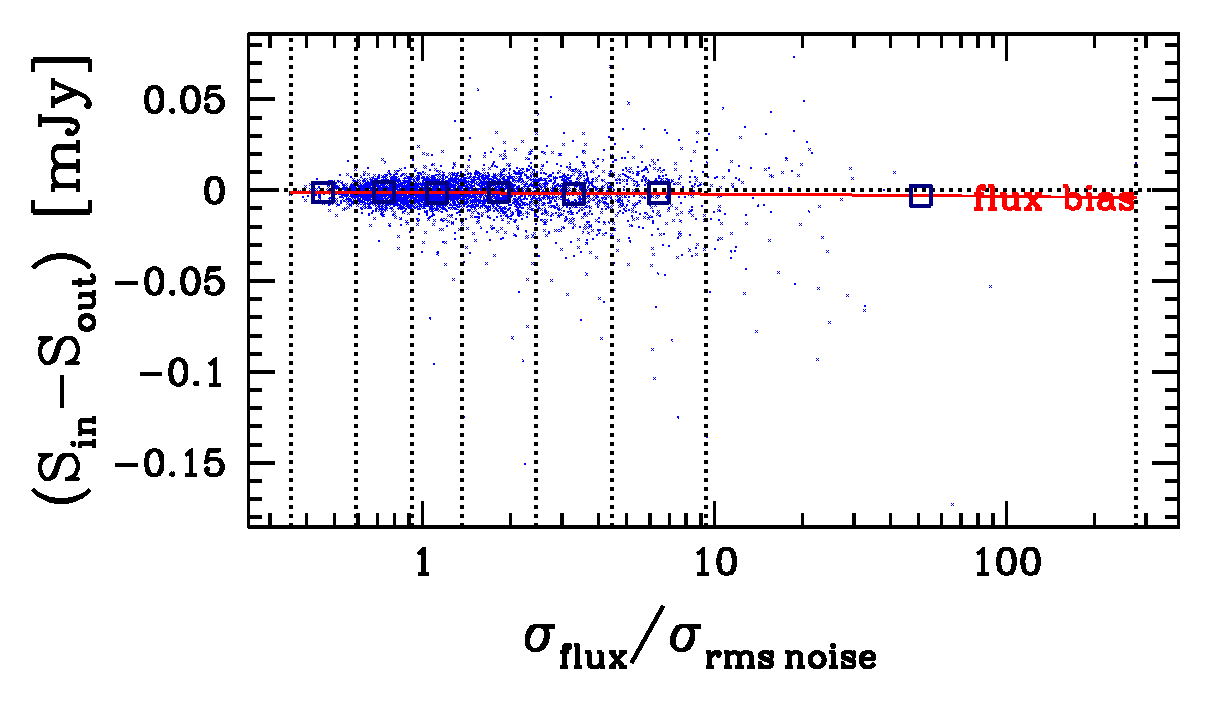
\includegraphics[width=0.8\textwidth]{galsim_24_fbias_1}
	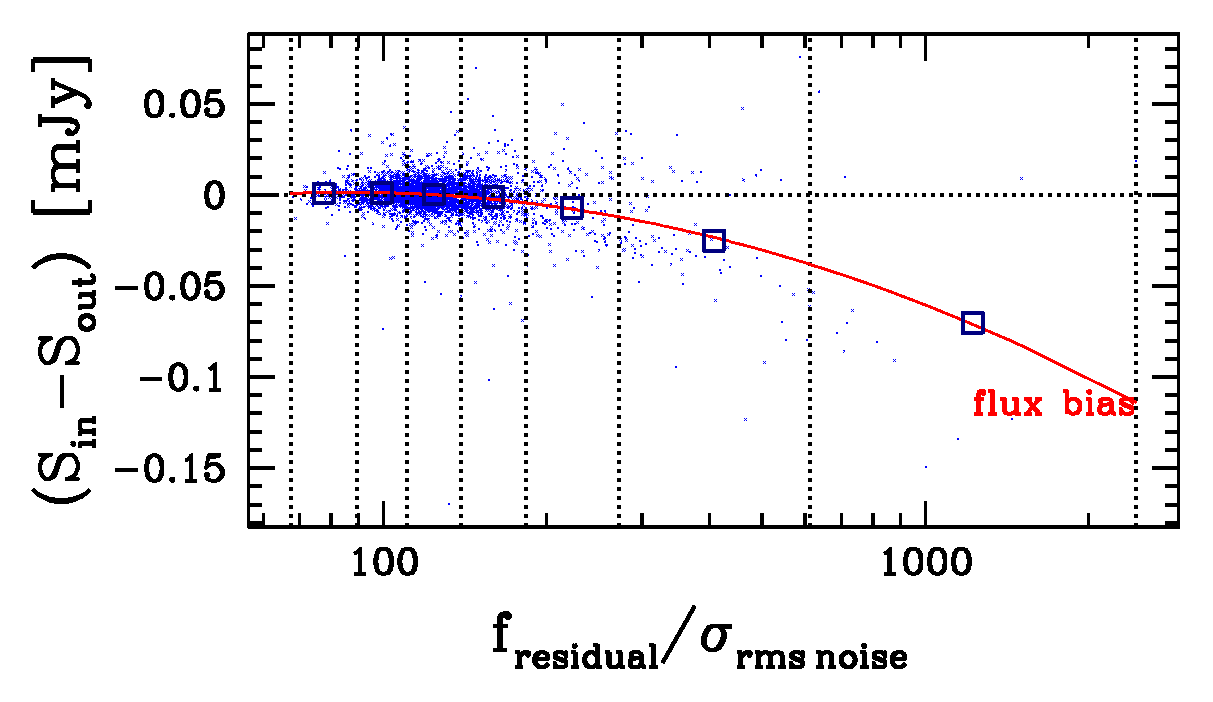
\includegraphics[width=0.8\textwidth]{galsim_24_fbias_2}
	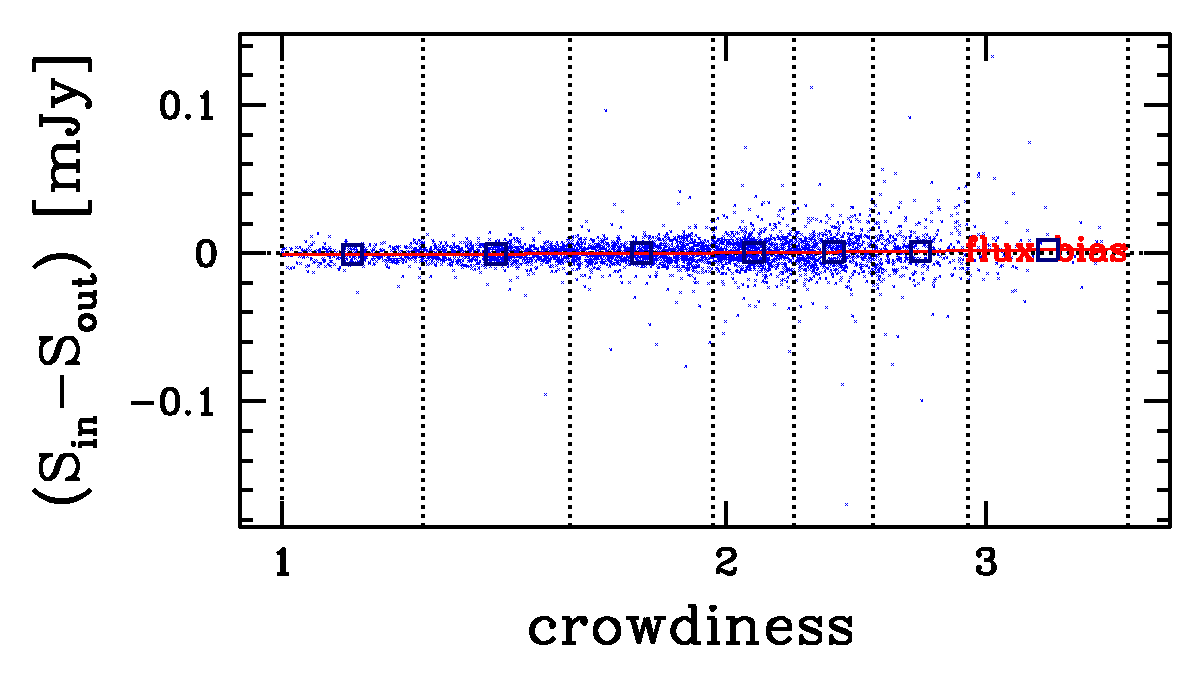
\includegraphics[width=0.8\textwidth]{galsim_24_fbias_3}
	\caption{Flux bias analysis from simulation.}
\end{figure}

\begin{figure}[H]
	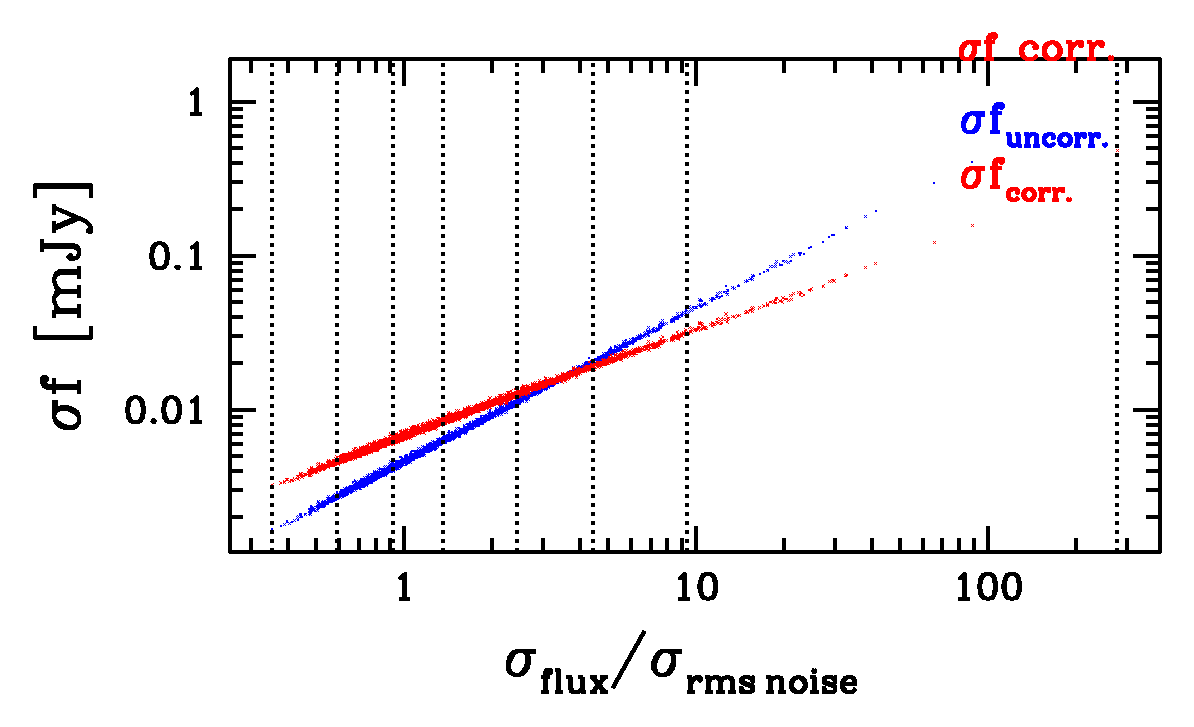
\includegraphics[width=0.8\textwidth]{galsim_24_dfcorr_1}
	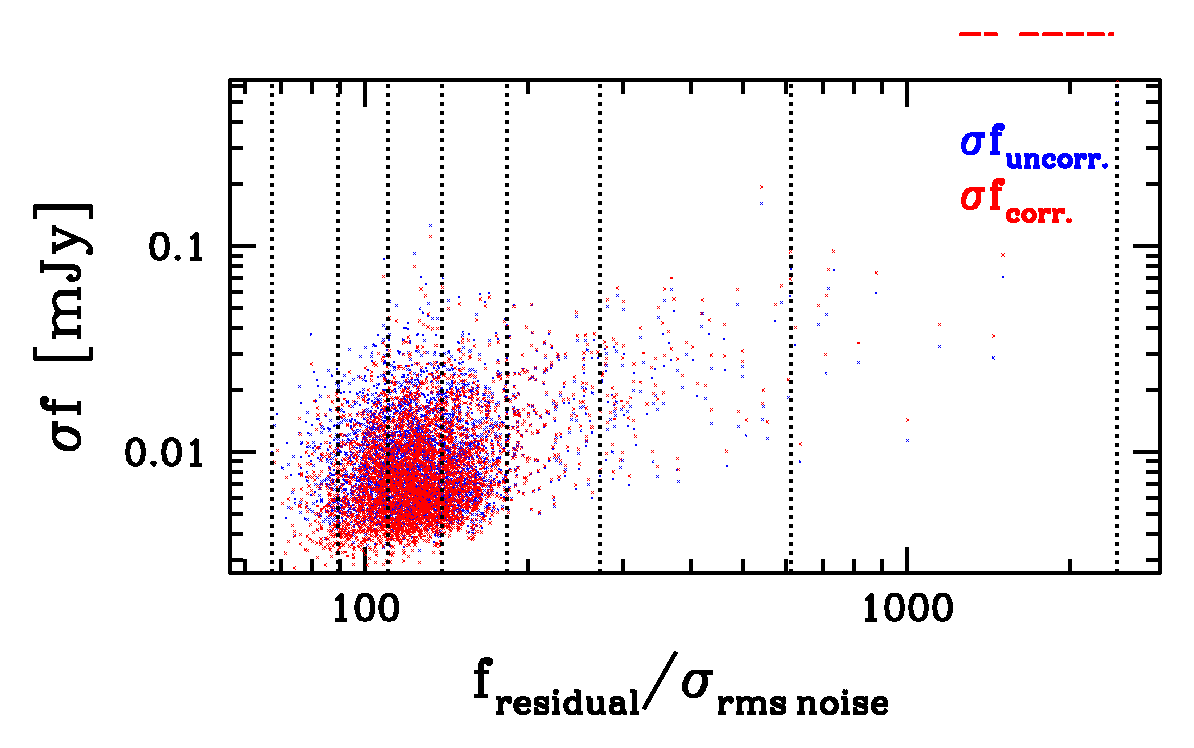
\includegraphics[width=0.8\textwidth]{galsim_24_dfcorr_2}
	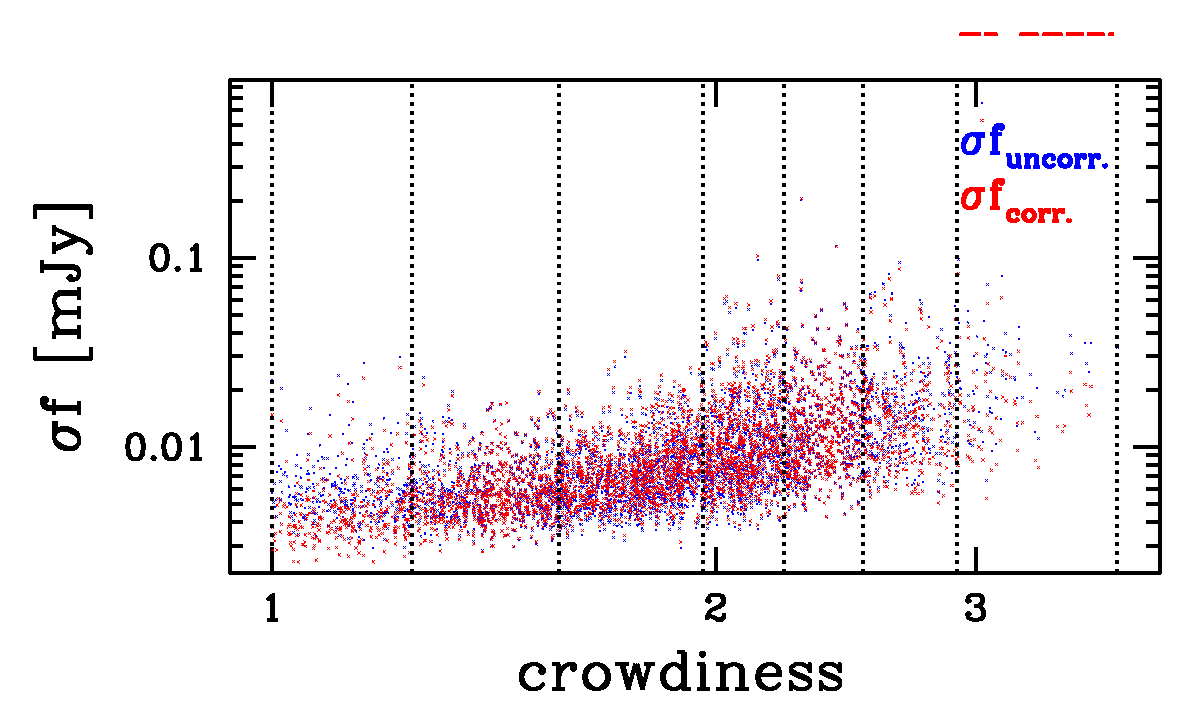
\includegraphics[width=0.8\textwidth]{galsim_24_dfcorr_3}
	\caption{Flux uncertainty analysis from simulation.}
\end{figure}

\begin{figure}[H]
	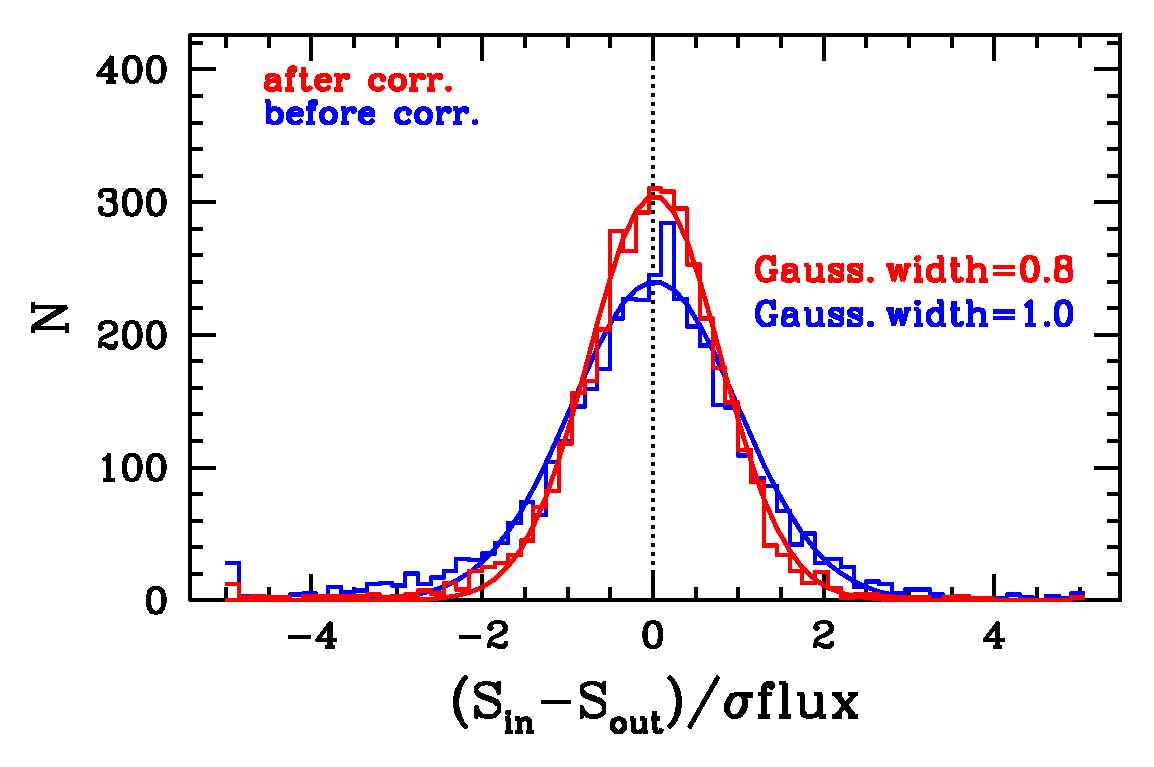
\includegraphics[width=0.75\textwidth]{galsim_24_hist_dfcorr_1}
	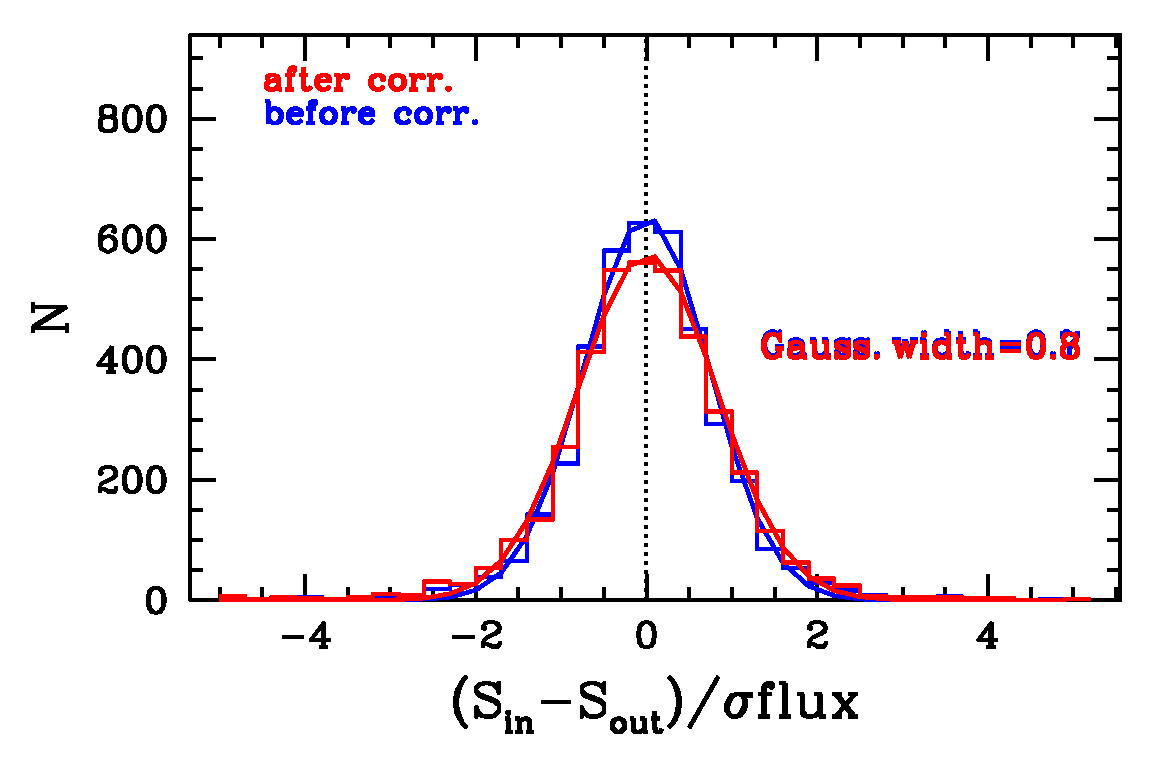
\includegraphics[width=0.75\textwidth]{galsim_24_hist_dfcorr_2}
	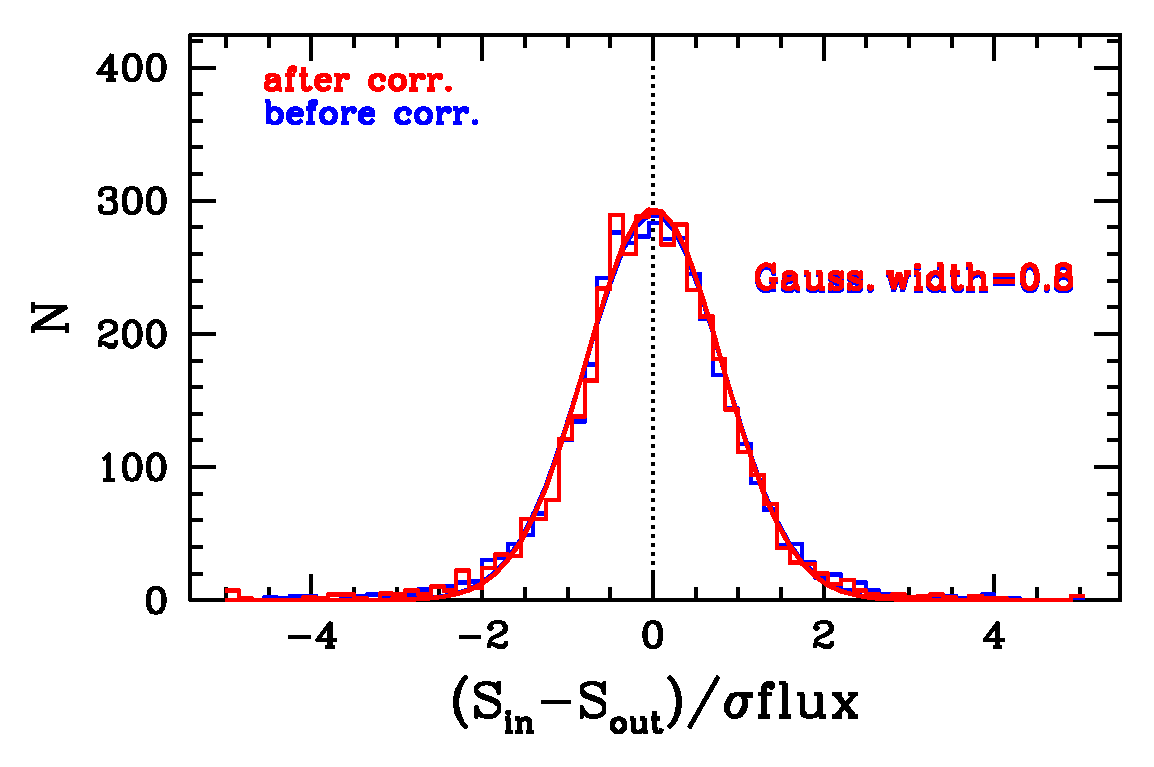
\includegraphics[width=0.75\textwidth]{galsim_24_hist_dfcorr_3}
	\caption{Statistical behavior of input minus output differences before and after correction.}
\end{figure}

%*************************************************************************************

\clearpage

%*************************************************************************************
\section{Band 20cm (Owen's map)}

\subsection{Galfit at band 20cm (Owen's map)}

We use these commands to run the galfit photometry at band 20cm:

\begin{lstlisting}[language=bash]
# run first-pass without varying source position
./do_Galfit 20cm 201500 -catalog irac_mips_fluxes_hdfn.dat
cd boxgalfit; do_GalfitRunqsub; cd ..
./do_Galfit 20cm 201500 -catalog irac_mips_fluxes_hdfn.dat -postparallel
# then second-pass varying source position
./do_Galfit 20cm 201500 -catalog irac_mips_fluxes_hdfn.dat -vary
cd boxgalfit_vary; do_GalfitRunqsub; cd ..
./do_Galfit 20cm 201500 -catalog irac_mips_fluxes_hdfn.dat -vary -postparallel
\end{lstlisting}

\subsection{Galsim at band 20cm (Owen's map)}

We use these commands to run the Monte-Carlo simulation at band 20cm:

\begin{lstlisting}[language=bash]
# first estimate magnitude range
# note that 20cm 3-sigma is about 7.5uJy (Owen's map)
load astroPhot.sm
convert_flux2mag goodsn 20cm $(0.0022*01) 1 # (mBias 0 fBias -5e-05) # => 10.5112
convert_flux2mag goodsn 20cm $(0.0022*25) 1 # (mBias 0 fBias -5e-05) # => 7.03979
# then do the simulation
./do_Galsim 20cm 201500 -mag0 7.03979 -mag1 10.5112 -number 6000 -vary \
-catalog irac_mips_fluxes_hdfn.dat
cd boxgalsim; do_GalsimRunqsub; cd ..
./do_Galsim 20cm 201500 -mag0 7.03979 -mag1 10.5112 -number 6000 -vary \
-catalog irac_mips_fluxes_hdfn.dat -postparallel
\end{lstlisting}

\subsection{Galsim Analysis at band 20cm (Owen's map)}

We use these commands to run the simulation analysis at band 20cm:

\begin{lstlisting}[language=bash]
cd doing20cm/
sm
macro read run_simu_stats_v7.sm run_simu_stats_v7 20cm 201500
\end{lstlisting}

Below are our statistical analyses:

\begin{figure}[H]
	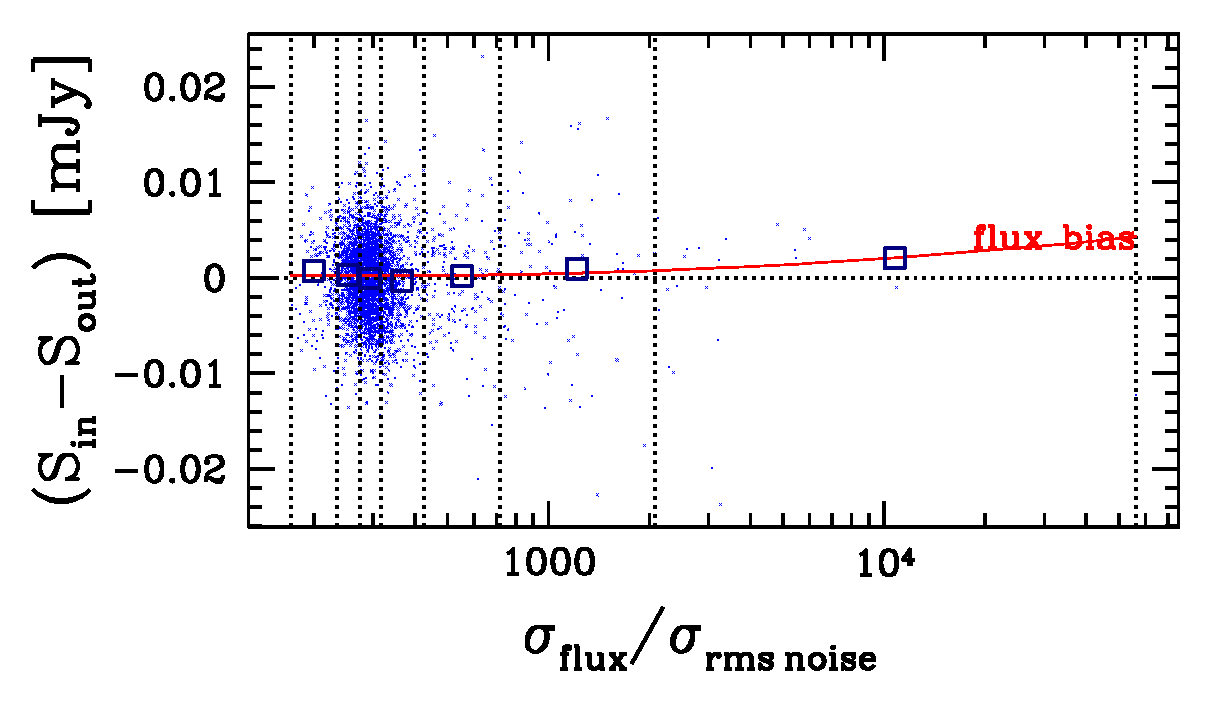
\includegraphics[width=0.8\textwidth]{galsim_20cm_fbias_1}
	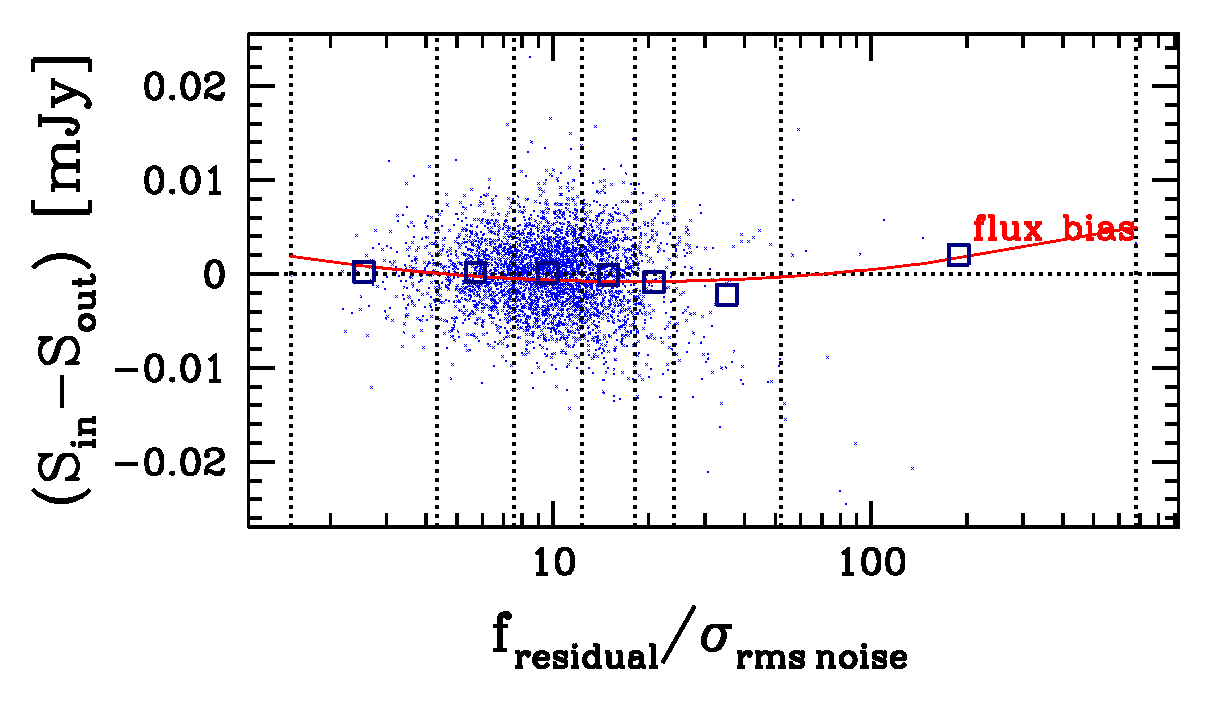
\includegraphics[width=0.8\textwidth]{galsim_20cm_fbias_2}
	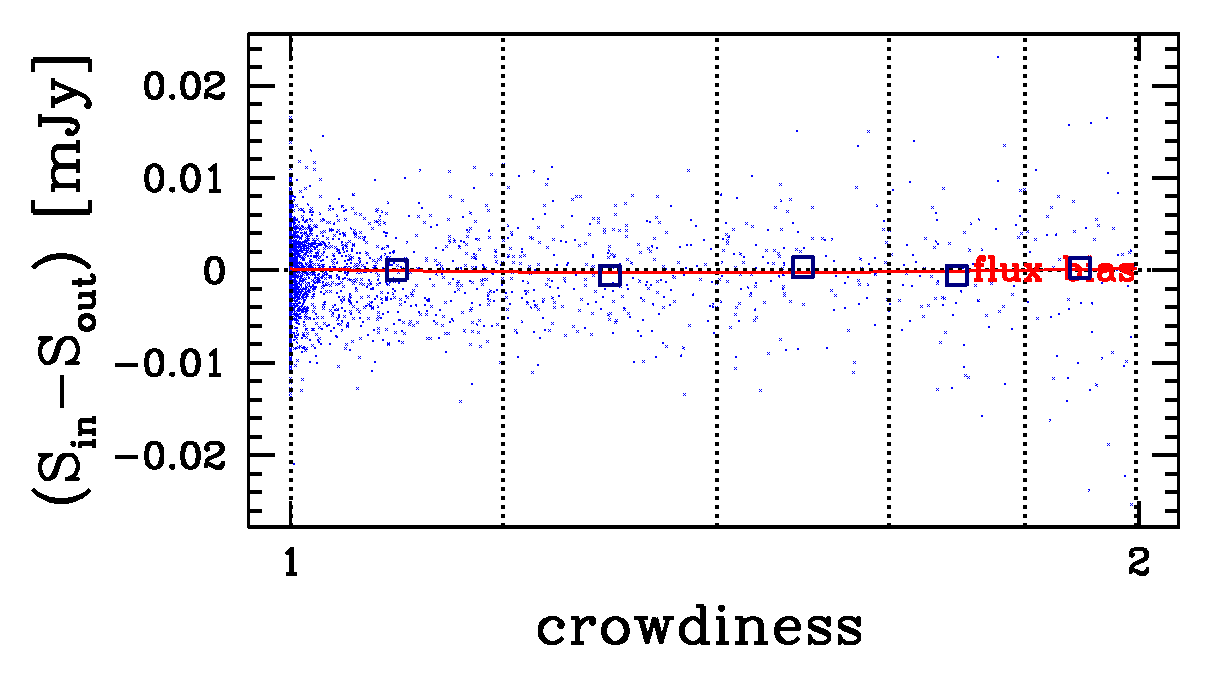
\includegraphics[width=0.8\textwidth]{galsim_20cm_fbias_3}
	\caption{Flux bias analysis from simulation.}
\end{figure}

\begin{figure}[H]
	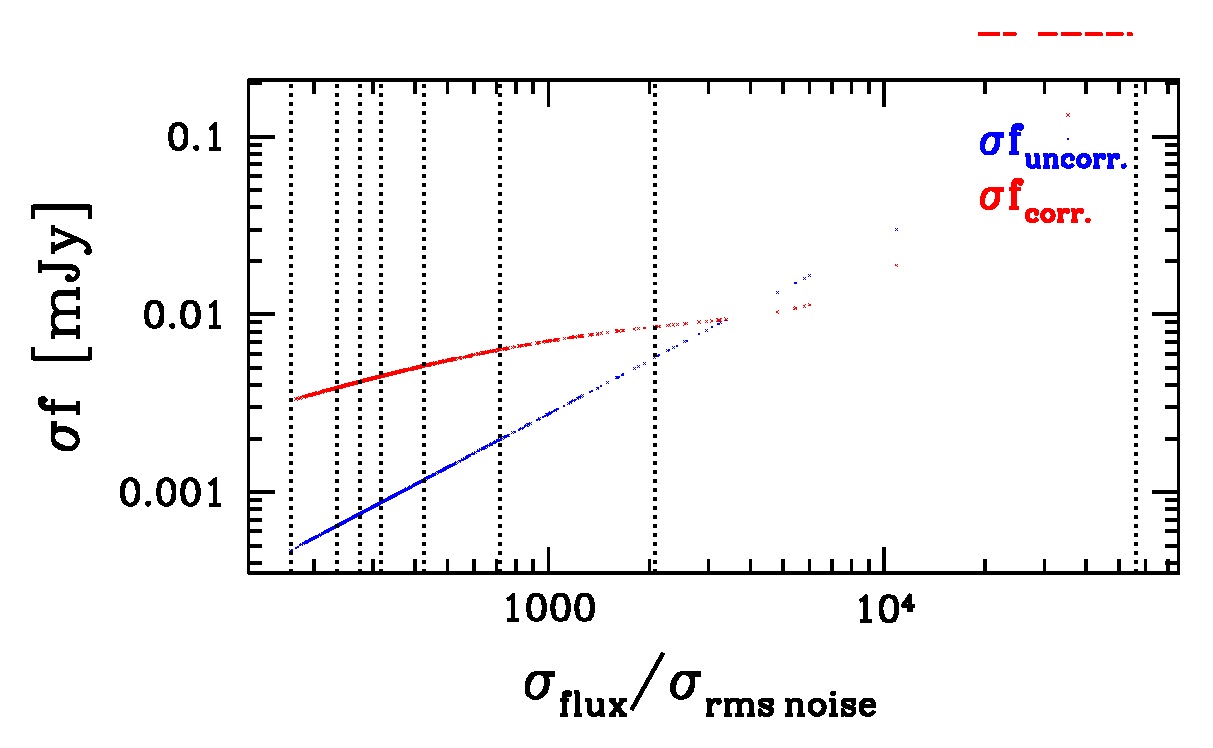
\includegraphics[width=0.8\textwidth]{galsim_20cm_dfcorr_1}
	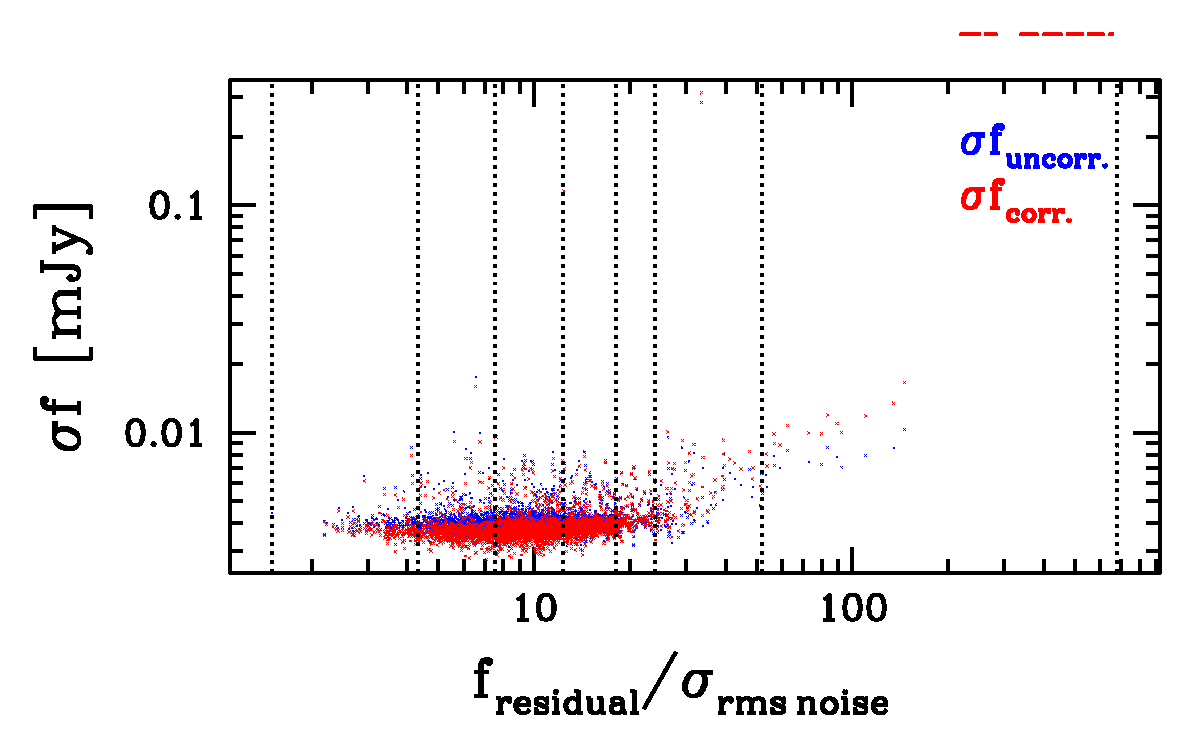
\includegraphics[width=0.8\textwidth]{galsim_20cm_dfcorr_2}
	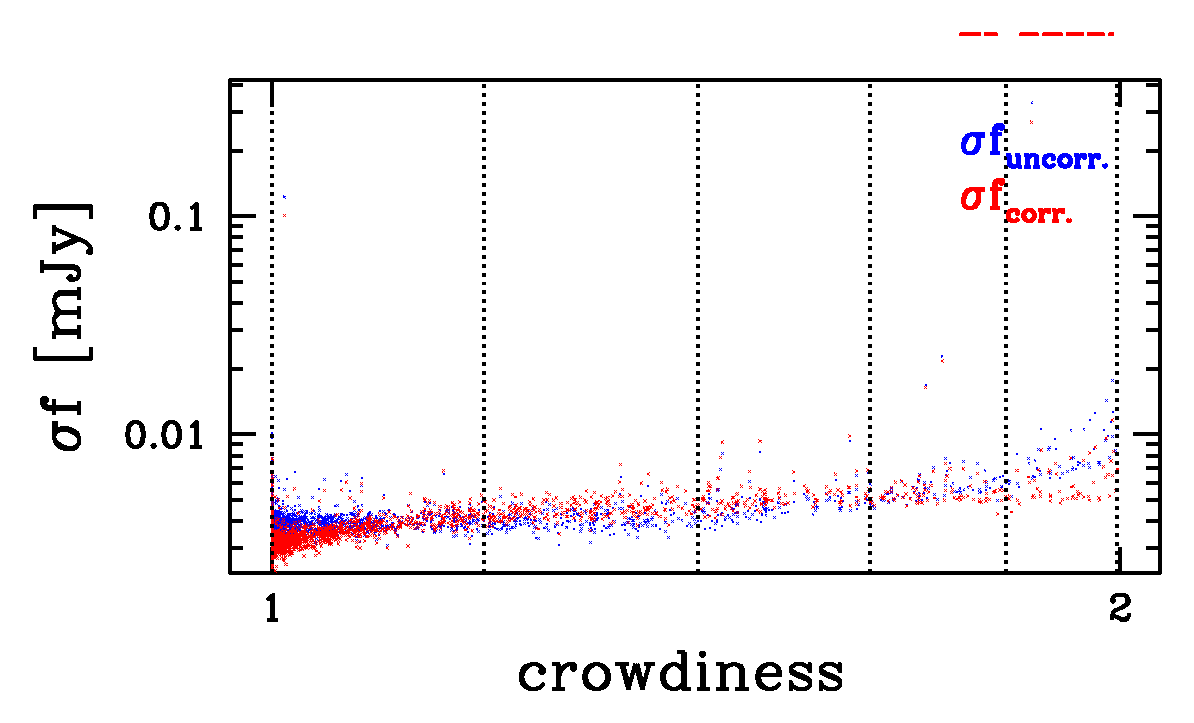
\includegraphics[width=0.8\textwidth]{galsim_20cm_dfcorr_3}
	\caption{Flux uncertainty analysis from simulation.}
\end{figure}

\begin{figure}[H]
	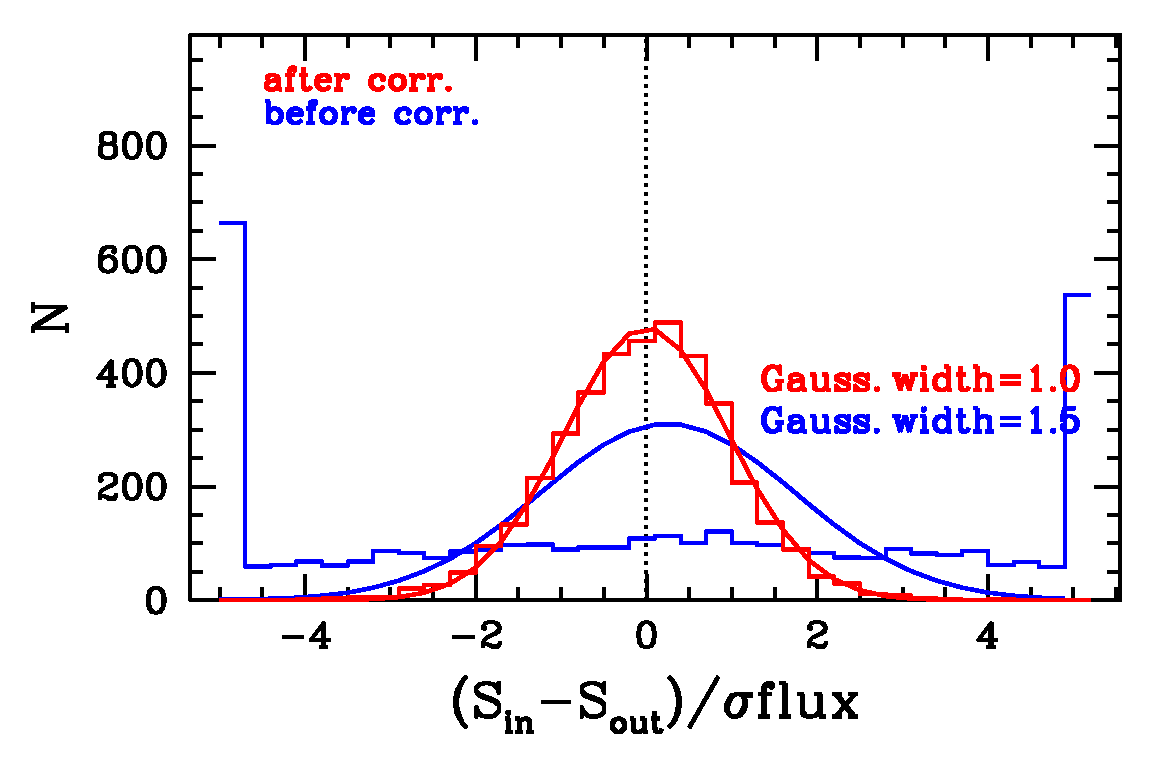
\includegraphics[width=0.75\textwidth]{galsim_20cm_hist_dfcorr_1}
	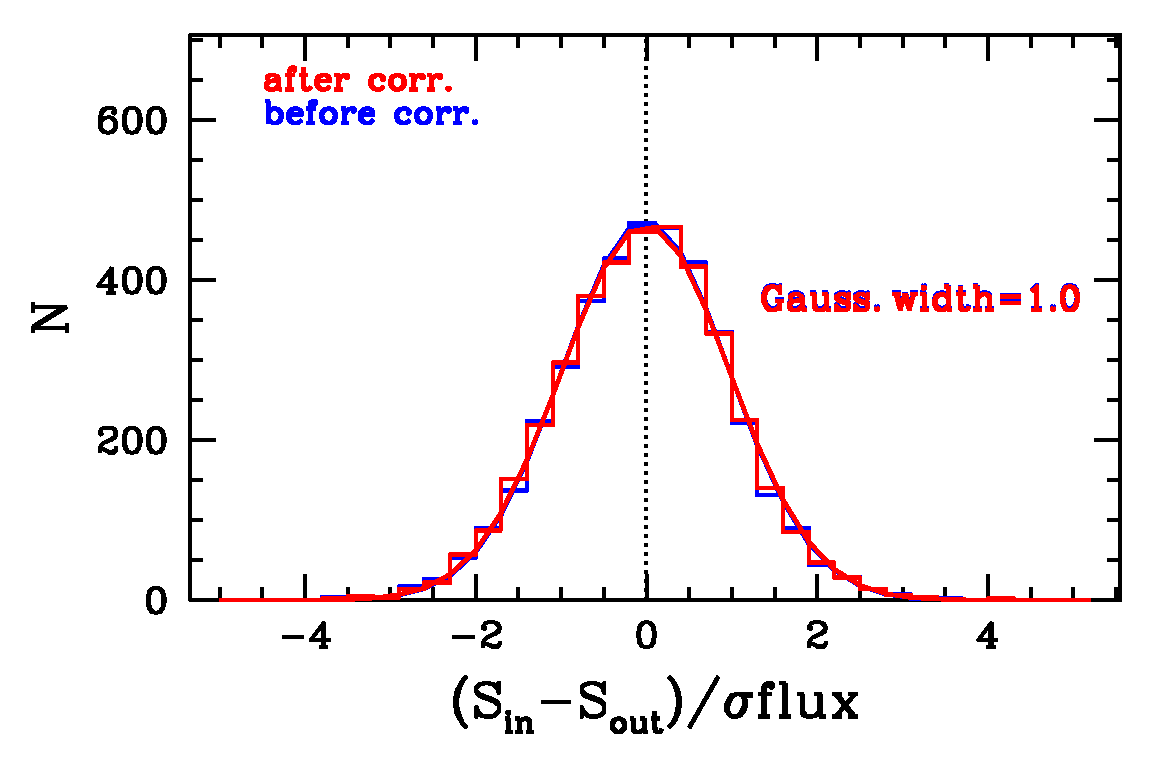
\includegraphics[width=0.75\textwidth]{galsim_20cm_hist_dfcorr_2}
	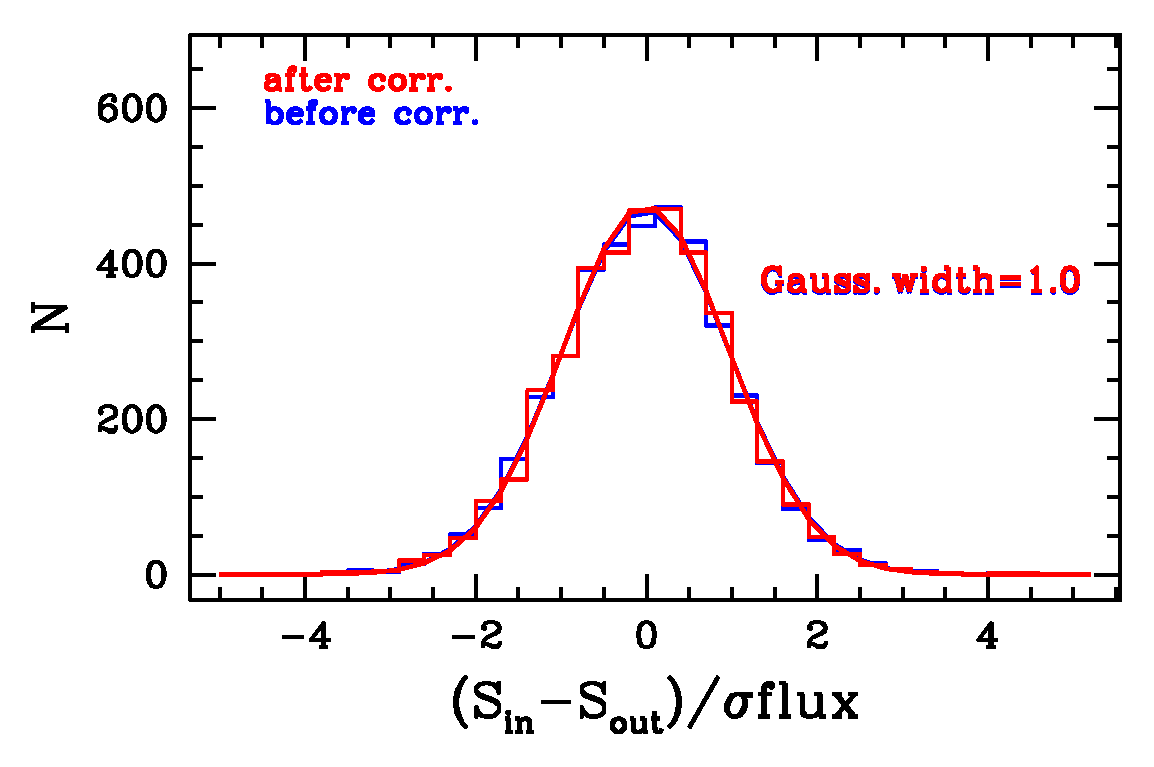
\includegraphics[width=0.75\textwidth]{galsim_20cm_hist_dfcorr_3}
	\caption{Statistical behavior of input minus output differences before and after correction.}
\end{figure}

\subsection{Compare with literature: Elbaz et al. 2013}

\begin{figure}[H]
	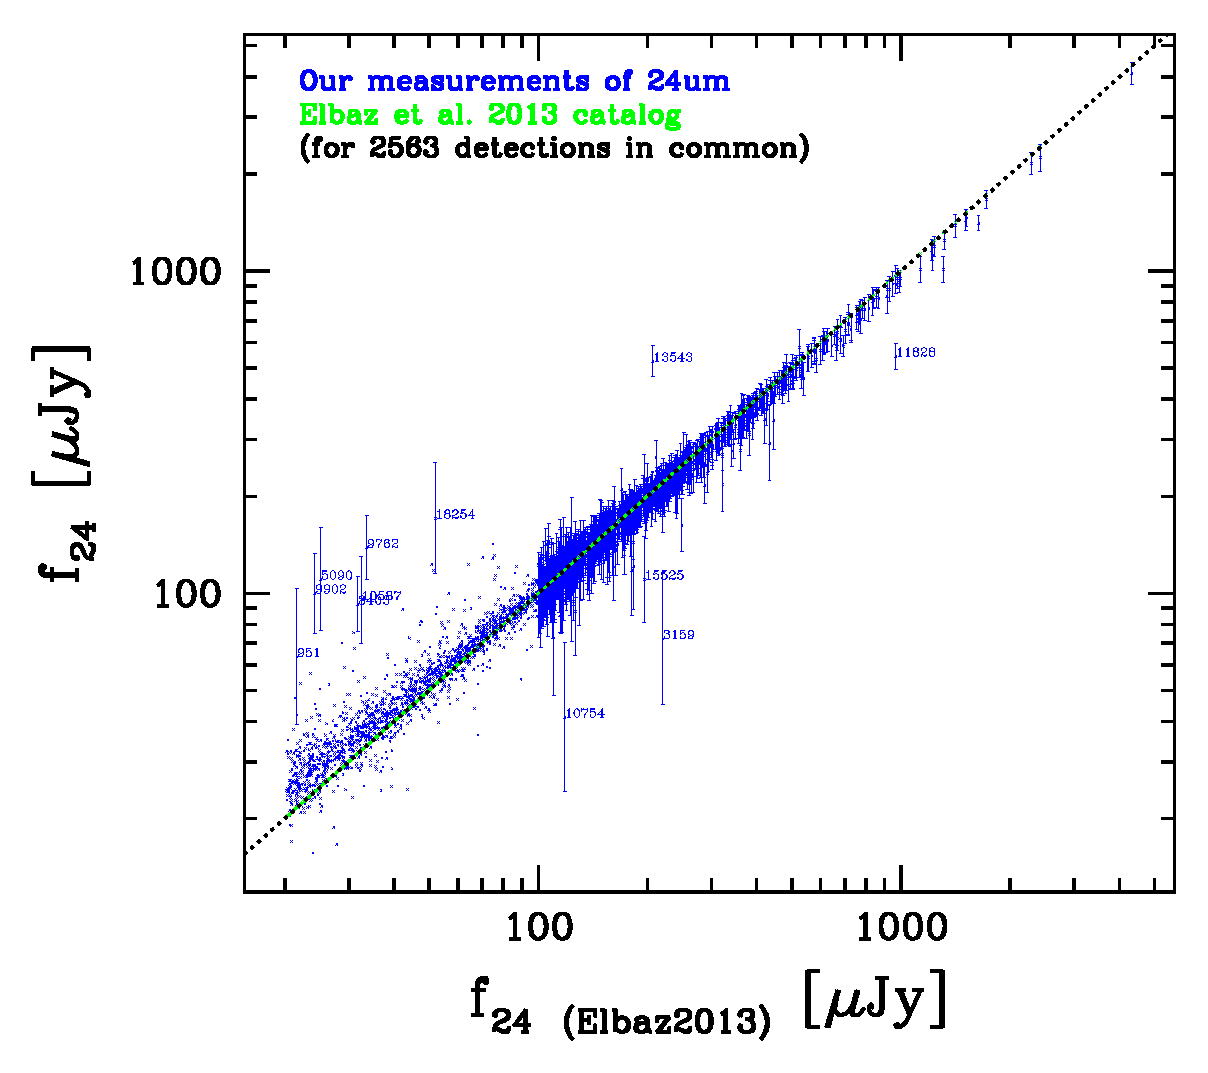
\includegraphics[width=0.95\textwidth]{Compare_measurments_of_24um_with_Elbaz_2013}
	\caption{Compare our final corrected 24${\mu}m$ measurements with the literature measurements of Elbaz et al. 2013 (\url{http://adsabs.harvard.edu/abs/2013yCat..35330119E}). Y axis is our measurements. A linear dashed green-black line indicates a one-to-one correlation. Details of the most outliers are given below: ID11828 is bright and extended, our PSF fitting could not recover its entire flux. ID13543 is bright and blended with its neighborhood ID13542 which is also bright. Not sure why and how to fix yet \textcolor{red}{(TODO)}. ID3159 and ID3119 are close within 2'' and the peak of flux at in between of them. ID10754 is only 15'' from the bright 20'' diameter spiral source ID10611, therefore got highly contaminated results. ID18254 and ID18253 are blended, and the latter one is brighter and likely extended, hence the former one got contaminated flux.}
\end{figure}

%*************************************************************************************

\clearpage

%*************************************************************************************
\section{Band 20cm (Morrison's map)}

\subsection{Galfit at band 20cm (Morrison's map)}

We use these commands to run the galfit photometry at band 20cm:

\begin{lstlisting}[language=bash]
# run first-pass without varying source position
./do_Galfit 20cm_Glenn 201500 -catalog irac_mips_fluxes_hdfn.dat
cd boxgalfit; do_GalfitRunqsub; cd ..
./do_Galfit 20cm_Glenn 201500 -catalog irac_mips_fluxes_hdfn.dat -postparallel
# then second-pass varying source position
./do_Galfit 20cm_Glenn 201500 -catalog irac_mips_fluxes_hdfn.dat -vary
cd boxgalfit_vary; do_GalfitRunqsub; cd ..
./do_Galfit 20cm_Glenn 201500 -catalog irac_mips_fluxes_hdfn.dat -vary -postparallel
\end{lstlisting}

\subsection{Galsim at band 20cm (Morrison's map)}

We use these commands to run the Monte-Carlo simulation at band 20cm:

\begin{lstlisting}[language=bash]
# first estimate magnitude range
# In Morrison et al. 2010 catalog, 1230 radio sources were detected. 
# Their median df20cm is ~10uJy, while minimum df20cm is ~3uJy. 
# Their minimum f20cm is ~21uJy, and maximum f20cm is ~263uJy. 
# Therefore we do simulation with f20cm from 10uJy to 263uJy. 
load astroPhot.sm
convert_flux2mag goodsn 20cm_Glenn 0.010 1 # (mBias 0 fBias 0) # => 9.6961
convert_flux2mag goodsn 20cm_Glenn 0.263 1 # (mBias 0 fBias 0) # => 6.14621
# then do the simulation
./do_Galsim 20cm_Glenn 201500 -mag0 6.14621 -mag1 9.6961 -number 6000 -vary \
-catalog irac_mips_fluxes_hdfn.dat
cd boxgalsim; do_GalsimRunqsub; cd ..
./do_Galsim 20cm_Glenn 201500 -mag0 6.14621 -mag1 9.6961 -number 6000 -vary \
-catalog irac_mips_fluxes_hdfn.dat -postparallel
\end{lstlisting}

\subsection{Galsim Analysis at band 20cm (Morrison's map)}

We use these commands to run the simulation analysis at band 20cm:

\begin{lstlisting}[language=bash]
cd doing20cm_Glenn/
sm
macro read run_simu_stats_v7.sm run_simu_stats_v7 20cm_Glenn 201500
\end{lstlisting}

Below are our statistical analyses:

\begin{figure}[H]
	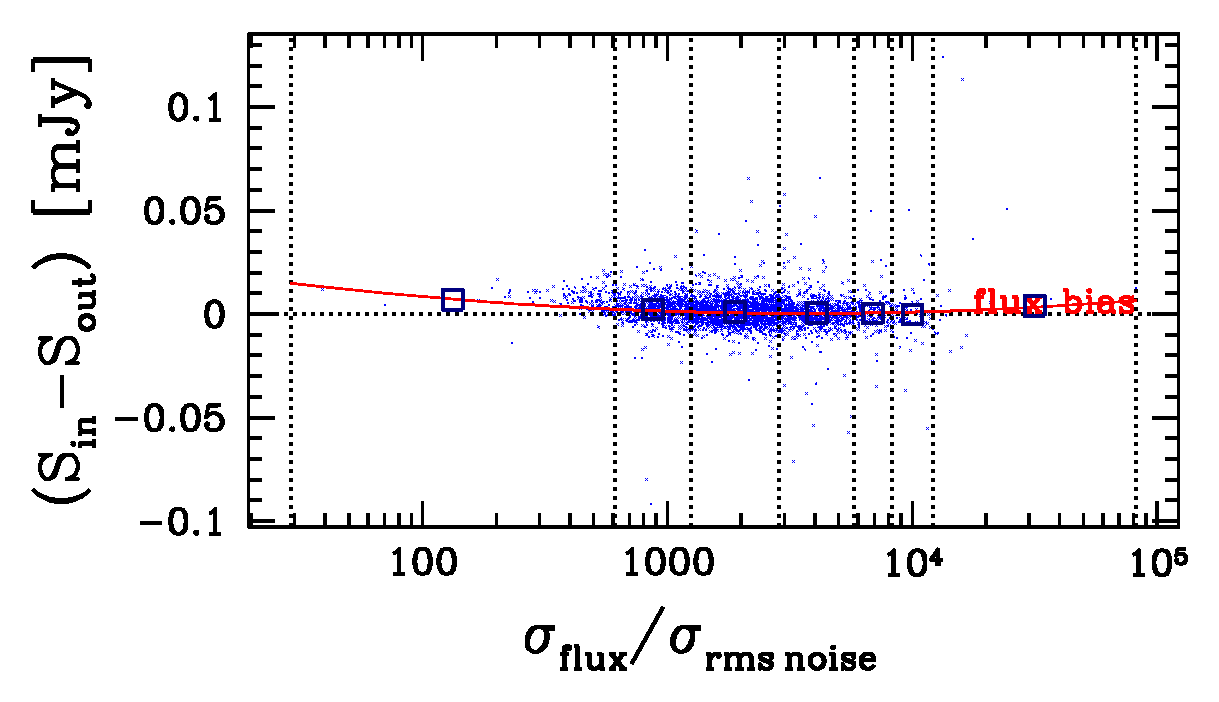
\includegraphics[width=0.8\textwidth]{galsim_20cm_Glenn_fbias_1}
	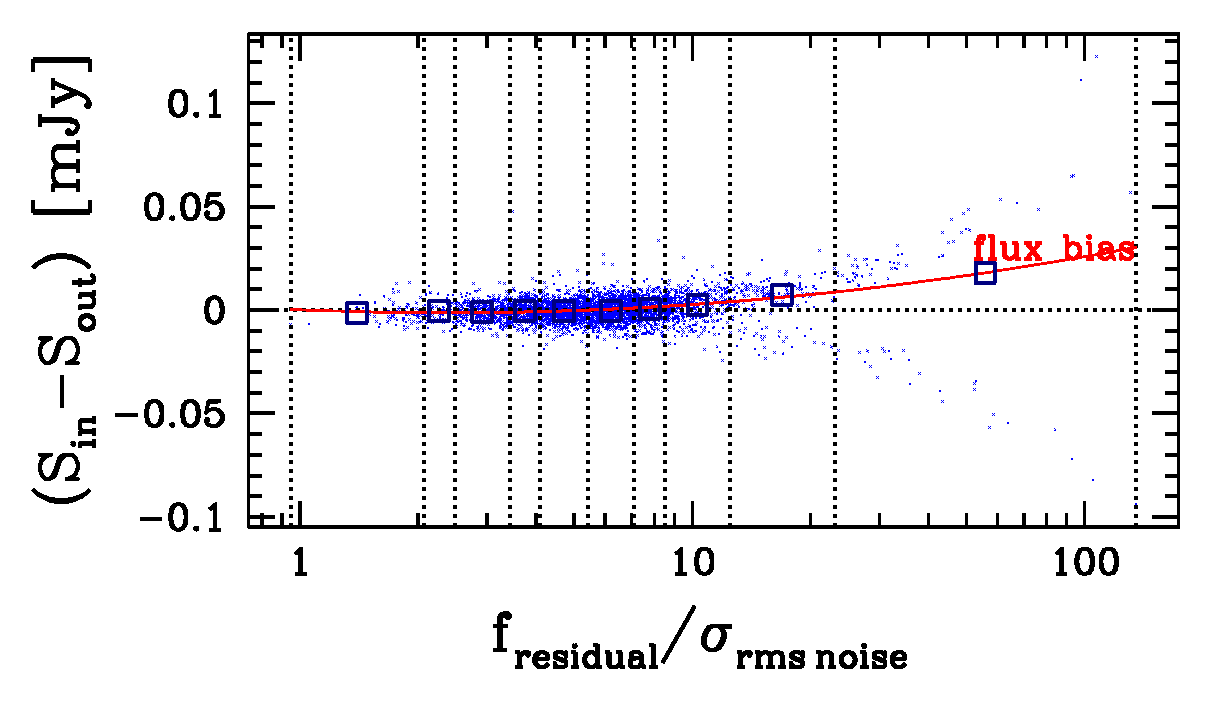
\includegraphics[width=0.8\textwidth]{galsim_20cm_Glenn_fbias_2}
	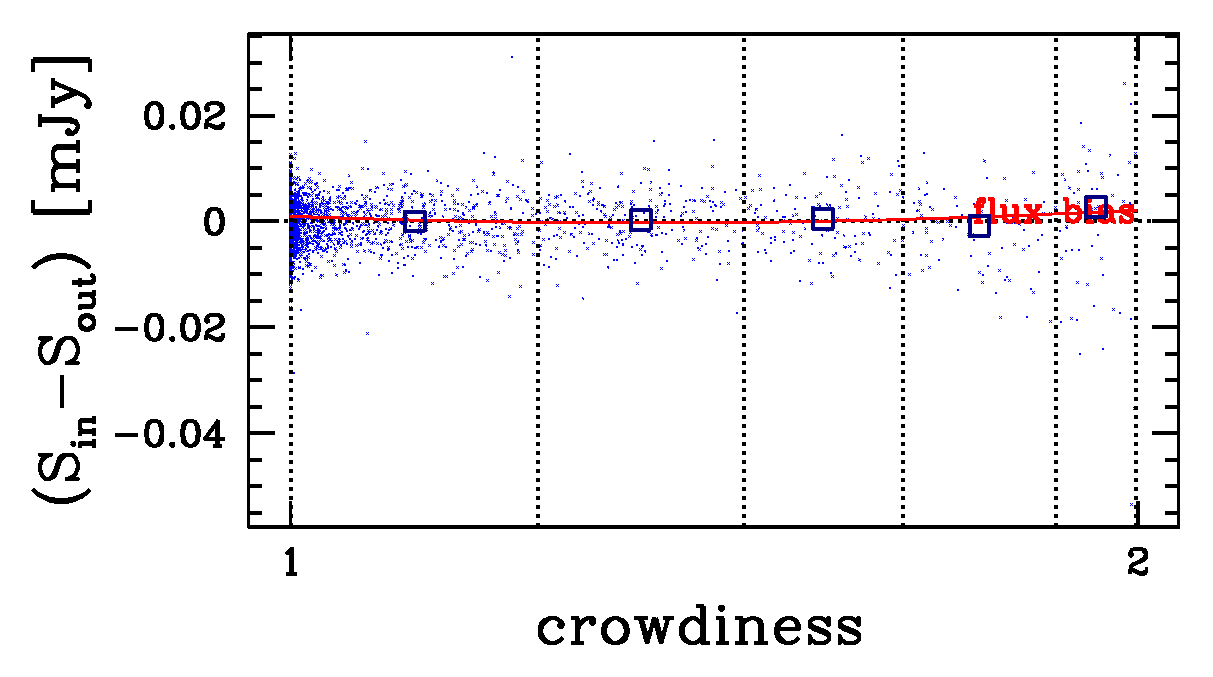
\includegraphics[width=0.8\textwidth]{galsim_20cm_Glenn_fbias_3}
	\caption{Flux bias analysis from simulation.}
\end{figure}

\begin{figure}[H]
	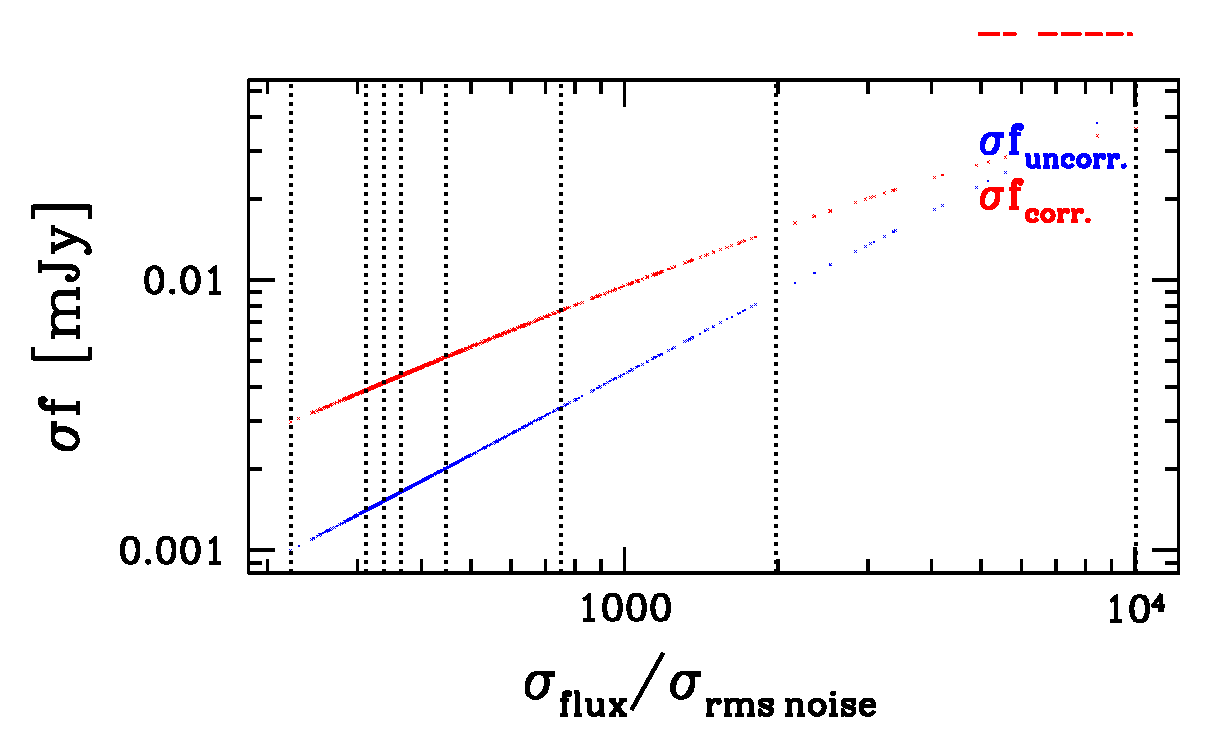
\includegraphics[width=0.8\textwidth]{galsim_20cm_Glenn_dfcorr_1}
	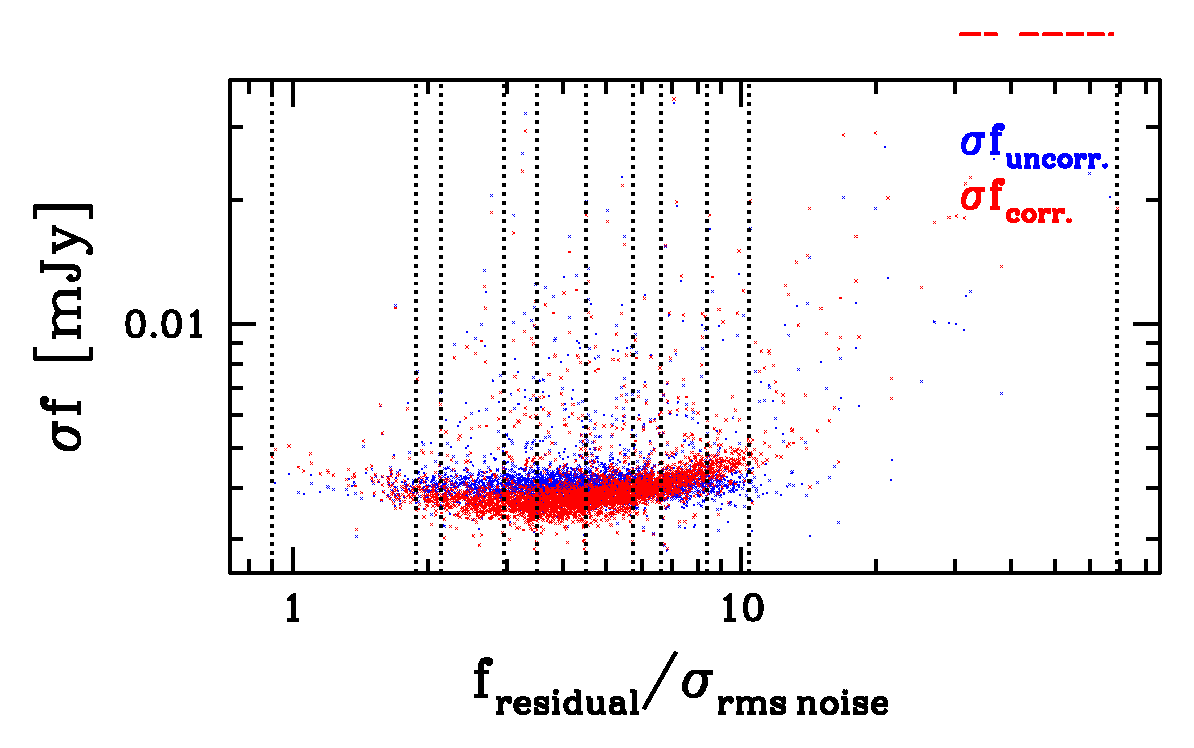
\includegraphics[width=0.8\textwidth]{galsim_20cm_Glenn_dfcorr_2}
	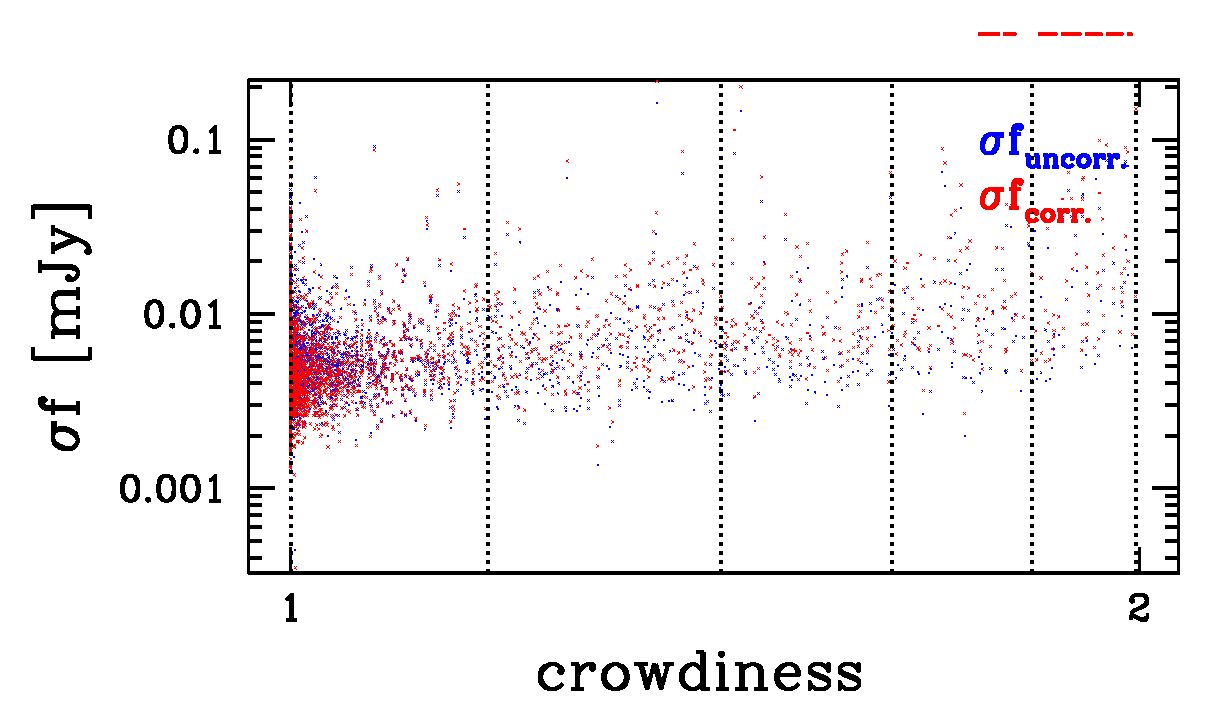
\includegraphics[width=0.8\textwidth]{galsim_20cm_Glenn_dfcorr_3}
	\caption{Flux uncertainty analysis from simulation.}
\end{figure}

\begin{figure}[H]
	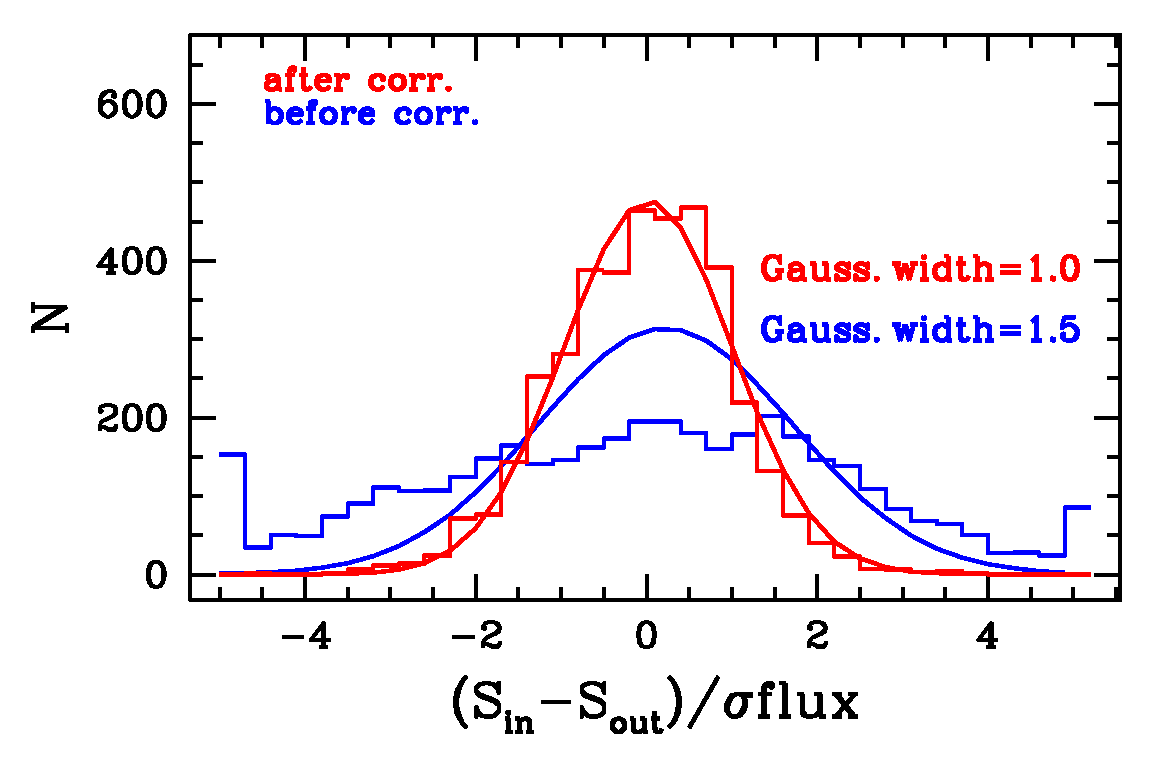
\includegraphics[width=0.75\textwidth]{galsim_20cm_Glenn_hist_dfcorr_1}
	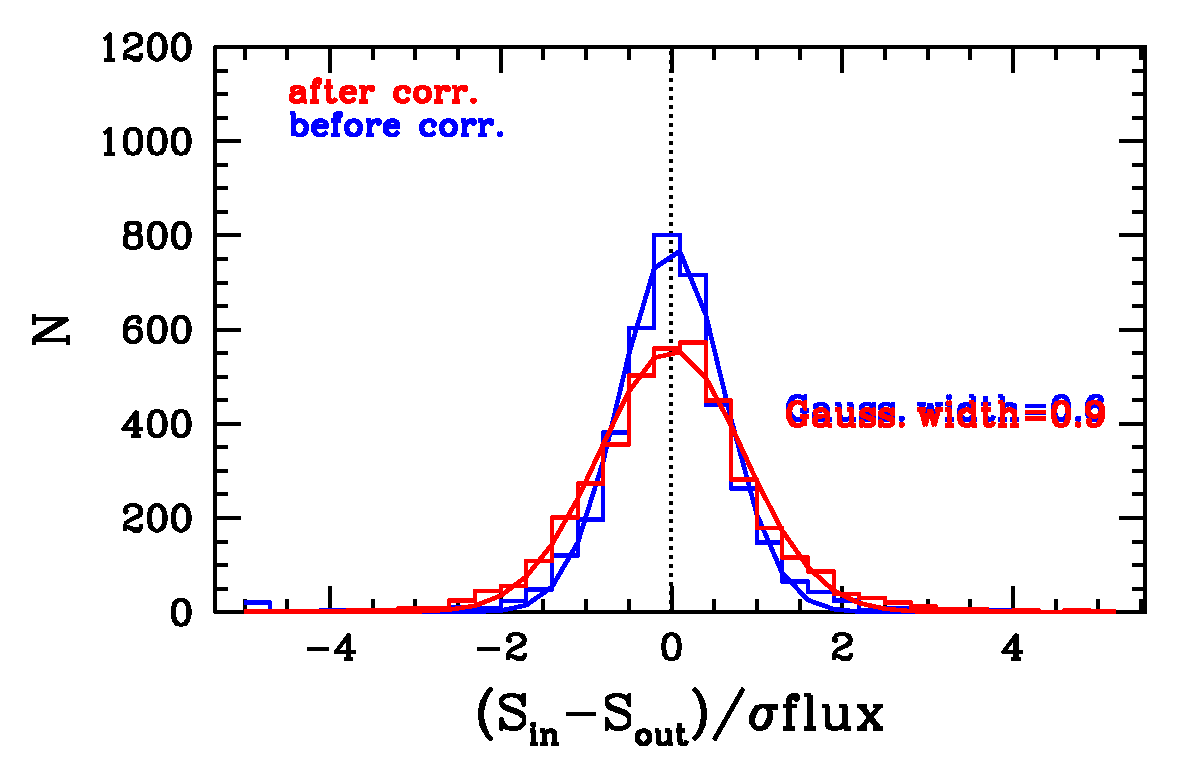
\includegraphics[width=0.75\textwidth]{galsim_20cm_Glenn_hist_dfcorr_2}
	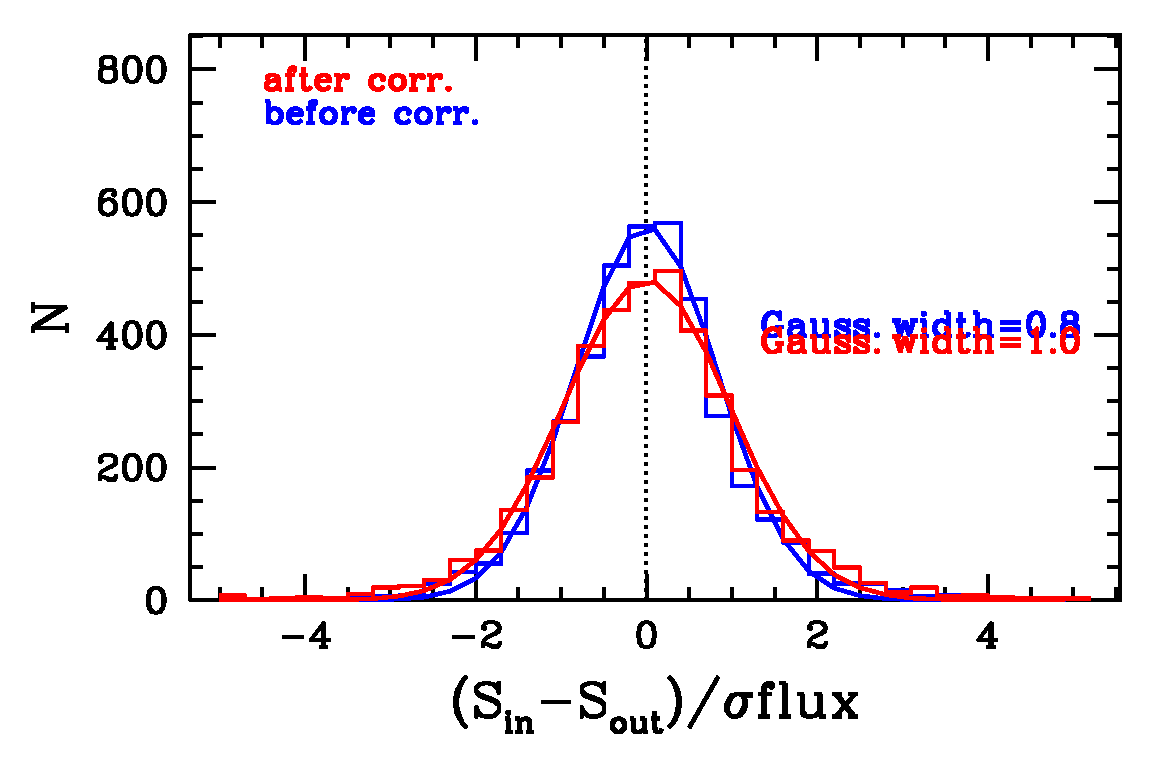
\includegraphics[width=0.75\textwidth]{galsim_20cm_Glenn_hist_dfcorr_3}
	\caption{Statistical behavior of input minus output differences before and after correction.}
\end{figure}

\subsection{Compare with literature: Morrison et al. 2010}

\begin{figure}[H]
	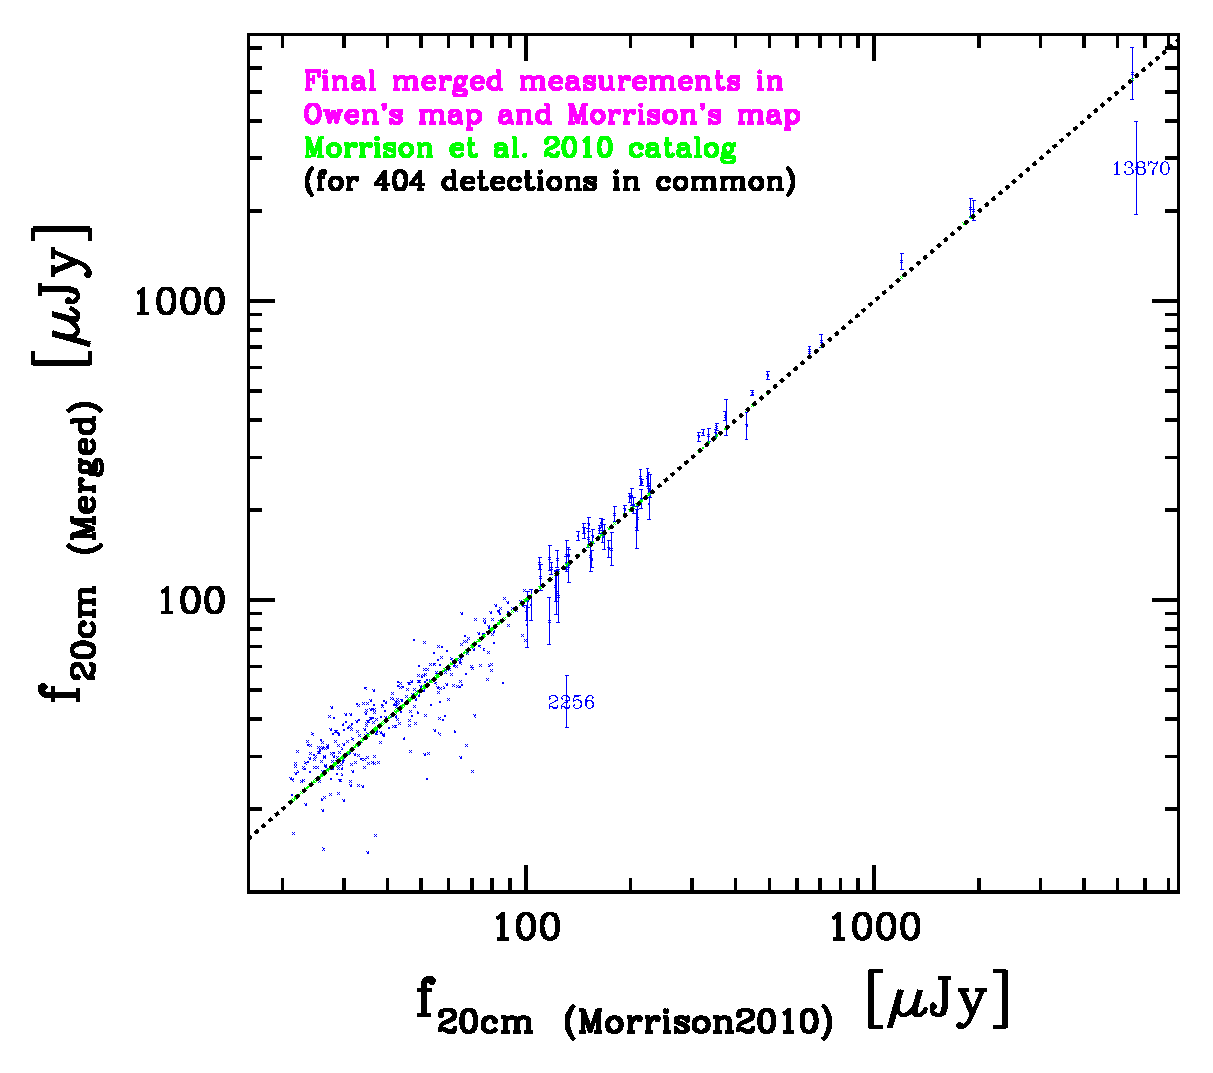
\includegraphics[width=0.95\textwidth]{Compare_measurments_of_20cm_with_Morrison_2010}
	\caption{Compare our two-radio-map-merged and sim-recipe-corrected 20cm measurements with the literature measurements in Morrison et al. 2010. Y axis is our measurements. A linear dashed green-black line indicates a one-to-one correlation. Details of several obvious outliers: ID13870 is an extremely bright radio source and has two peaks, likely two interacting components? ID2256 is relatively bright but heavily extended, and what we are fitting is PSF for now, hence could not recover its entire flux.}
\end{figure}



%*************************************************************************************
\end{document}